\begin{center}
  \large{\textsc{Измерение плотности человека. }}
\end{center}

\textbf{Состав:} Антон Грудкин, Николай Капралов, Антон
Егоров, Юрий Серов (все --- 9 класс), Андрей Йона (7 класс).

\textbf{Цель исследования:} измерить плотность человека. 

\textbf{Оборудование:} человек, озеро, пакет, песок, миски, весы, стаканчики.

\textbf{Методика исследования:} подбирается такая масса песка, что
человек, взяв её с собой под воду на вдохе, будет иметь нулевую
плавучесть. Этот объем и масса песка меряется весами и
стаканчиками. Затем плотность человека рассчитывается по формуле

\begin{equation}
  \label{eq:bz09_01}
  P = \frac{M \rho_{\text{в}}}{M + m - \rho_{\text{в}} V},
\end{equation}
где $M$~---~масса человека, $\rho_{\text{в}}$~---~плотность воды,
$m$~---~масса песка, $V$~---~объём песка. 

\begin{center}
  \textbf{Обоснование методики.}  
\end{center}

\begin{figure}[ht]
  \centering
  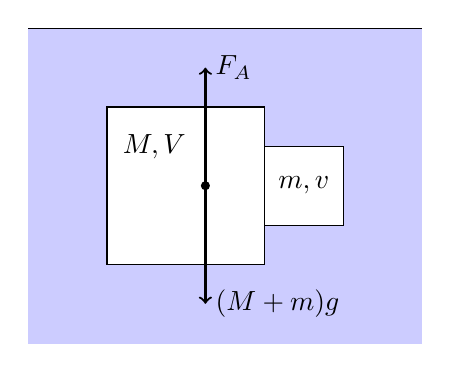
\begin{tikzpicture}
    \draw[fill=blue!20,draw=blue!20] (0,4) rectangle (5,0);
    \draw (0,4) -- +(5,0);
    \draw[fill=white] (1,3) rectangle ++(2,-2);
    \draw[fill=white] (3,2.5) rectangle ++(1,-1);
    \draw[thick,->] (2.25,2) -- +(0,-1.5) node[right] {$(M+m)g$};
    \draw[fill=black] (2.25,2) circle (0.05);
    \draw[thick,->] (2.25,2) -- +(0,1.5) node[right] {$F_A$};
    \draw (1.6,2.5) node {$M,V$};
    \draw (3.5,2) node {$m,v$};
  \end{tikzpicture}  
  \caption{К обоснованию методики.}
  \label{fig:bz09_density}
\end{figure}

Из рисунка видно, что $(M+m)g=F_A$, $F_A = \rho_{\text{в}} (V+v)
g$. Отсюда получаем, что
\begin{equation}
  \label{eq:bz09_1}
  V= \frac{M+m-\rho_{\text{в}} v} {\rho_{\text{в}}}.
\end{equation}

И находим плотность человека: 

\begin{equation}
  \label{eq:bz09_2}
  \rho = \frac{M}{V} = \frac{M \rho_{\text{в}}} {M+m-\rho_{\text{в}} v}.
\end{equation}

\begin{center}
  \textbf{Измерения.}  
\end{center}
\begin{table}[h]
  \centering
  \label{tbl:bz09_1}
  \begin{tabular}{|c|c|c|c|c|c|c|}
    \hline
    {} & $M$, кг & $m$, кг & $v,\unit{дм}^3$ & $V,\unit{дм}^3$ &
    $\rho_{\text{в}},\unit{кг/м}^3$ & $\rho, \unit{кг/м}^3$ \\
    \hline
    1 & 73 & 4,25 & 2 & 75,25 & 1000 & 970\\
    \hline
    2 & 52 & 1,7 & 0,8 & 52,9 & 1000 & 983\\
    \hline
    3 & 58 & 2,125 & 1 & 59,125 & 1000 & 981\\
    \hline
  \end{tabular}
\end{table}

\textbf{Погрешность:} при измерении объёма песка $\pm 10\unit{см}^3$,
при измерении массы песка $\pm 10 \unit{г}$, плотность воды $\pm 5
\unit{кг/м}^3$, масса человека $\pm 5 \unit{кг}$. 

Итого, с учётом погрешностей, получаем: $\rho=978 \pm 131
\unit{кг/м}^3$. 

%%% Local Variables: 
%%% mode: latex
%%% TeX-master: "../../report"
%%% End: 
